\section{Auswertung}
\subsection{Kontrastmessung}
Zunächst muss für eine bessere Qualität der späteren Messung der Kontrast
ermittelt werden. Dazu wird zunächst das Interferometer justiert und dann eine
Doppel-Glasplatte in das Interferometer eingebaut. Zwei Photodioden messen dann
 von der Intensität abhängige Spannungen. Die Spannungen werden dann von einem
Gerät in eine Differenzspannung umgewandelt und angezeigt. Dann wird der
Polarisationswinkel geändert und jeweils die maximale und minimale Differenz
ermittelt. Mit Hilfe von Formel \eqref{eqn:kontrast} wird dann der Kontrast
berechnet. Die gemessenen Spannungen mit den zugehörigen Winkeln werden in
Tabelle \ref{tab:kontrast} dargestellt.

\begin{table}
[H]
  \centering
\begin{tabular}{cccc}

  \toprule
$\phi \ [\si{\degree}]$ & $U_\text{min} \ [\SI{}{\volt}]$ &
$U_\text{max} \ [\SI{}{\volt}]$ & $K$ \\
\midrule

195 & \SI{1.28}{} & \SI{2.70}{} & \SI{0.36}{} \\

180 & \SI{1.52}{} & \SI{1.82}{} & \SI{0.09}{} \\

165 & \SI{0.76}{} & \SI{2.01}{} & \SI{0.45}{} \\

150 & \SI{0.24}{} & \SI{1.70}{} & \SI{0.75}{} \\

135 & \SI{0.06}{} & \SI{1.30}{} & \SI{0.91}{} \\

120 & \SI{0.10}{} & \SI{0.95}{} & \SI{0.81}{} \\

105 & \SI{0.26}{} & \SI{0.82}{} & \SI{0.52}{} \\

90  & \SI{0.67}{} & \SI{0.81}{} & \SI{0.09}{} \\

75  & \SI{0.47}{} & \SI{1.57}{} & \SI{0.54}{} \\

60  & \SI{0.15}{} & \SI{2.66}{} & \SI{0.89}{} \\

45  & \SI{0.14}{} & \SI{3.41}{} & \SI{0.92}{} \\

30  & \SI{0.54}{} & \SI{3.13}{} & \SI{0.71}{} \\

15  & \SI{1.21}{} & \SI{2.75}{} & \SI{0.39}{} \\

0   & \SI{1.64}{} & \SI{1.90}{} & \SI{0.07}{} \\

-15 & \SI{0.70}{} & \SI{2.00}{} & \SI{0.48}{} \\

\bottomrule
\end{tabular}

\caption{Berechneter Kontrast in Abhängigkeit der Polarisationsrichtung}
\label{tab:kontrast}
\end{table}



Nach Auftragen der Messwerte kann auf einen Zusammenhang schließen, der der
Betragsfunktion des Sinus ähnelt. Die Ausgleichsfunktion lautet somit
\begin{equation}
  f(\phi) = a \cdot \lvert \sin(b \cdot \phi +c) \rvert +d
\end{equation}
Die Messwerte und die Ausgleichsfunktion sind in Abbildung \ref{fig:kontrast}
dargestellt.

Für die Parameter ergeben sich die folgenden Werte
\begin{align*}
  a &= 0.88 \pm 0.05 \\
  b &= \SI{2.00 \pm 0.02}{\per\radian} \\
    &\hat{=}\, \SI{114.82 \pm 1.03}{\per\degree} \\
  c &= -0.06 \pm 0.04 \\
  d &= 0.03 \pm 0.03 \\
\end{align*}

Der Parameter $a$ beschreibt die Amplitude, $b$ eine Frequenz, $c$ die
Phasenverschiebung und $d$ den Kontrastoffset.
Zur Berechnung des optimalen Polarisationswinkel wird das Maximum der
Ausgleichsfunktion ermittelt.
\begin{equation}
  \phi = \frac{1}{b} \left(\frac{\pi}{2} -c \right)
\end{equation}
Dadurch ergibt sich ein Winkel von
\begin{align*}
  \phi &= \SI{0.82}{\radian} \\
       &\hat{=} \, \SI{46.72}{\degree} \\
\end{align*}
Der Fehler berechnet sich mit Hilfe der Gaußschen Fehlerfortpflanzung
\begin{equation}
  \Delta \phi =\sqrt{\left(- \frac{1}{b^2} \left(\frac{\pi}{2} -c \right)  \right)^2
  \Delta b^2 + \left(- \frac{1}{b}\right)^2 \Delta c^2}
\end{equation}

\begin{figure}[H]
  \centering
  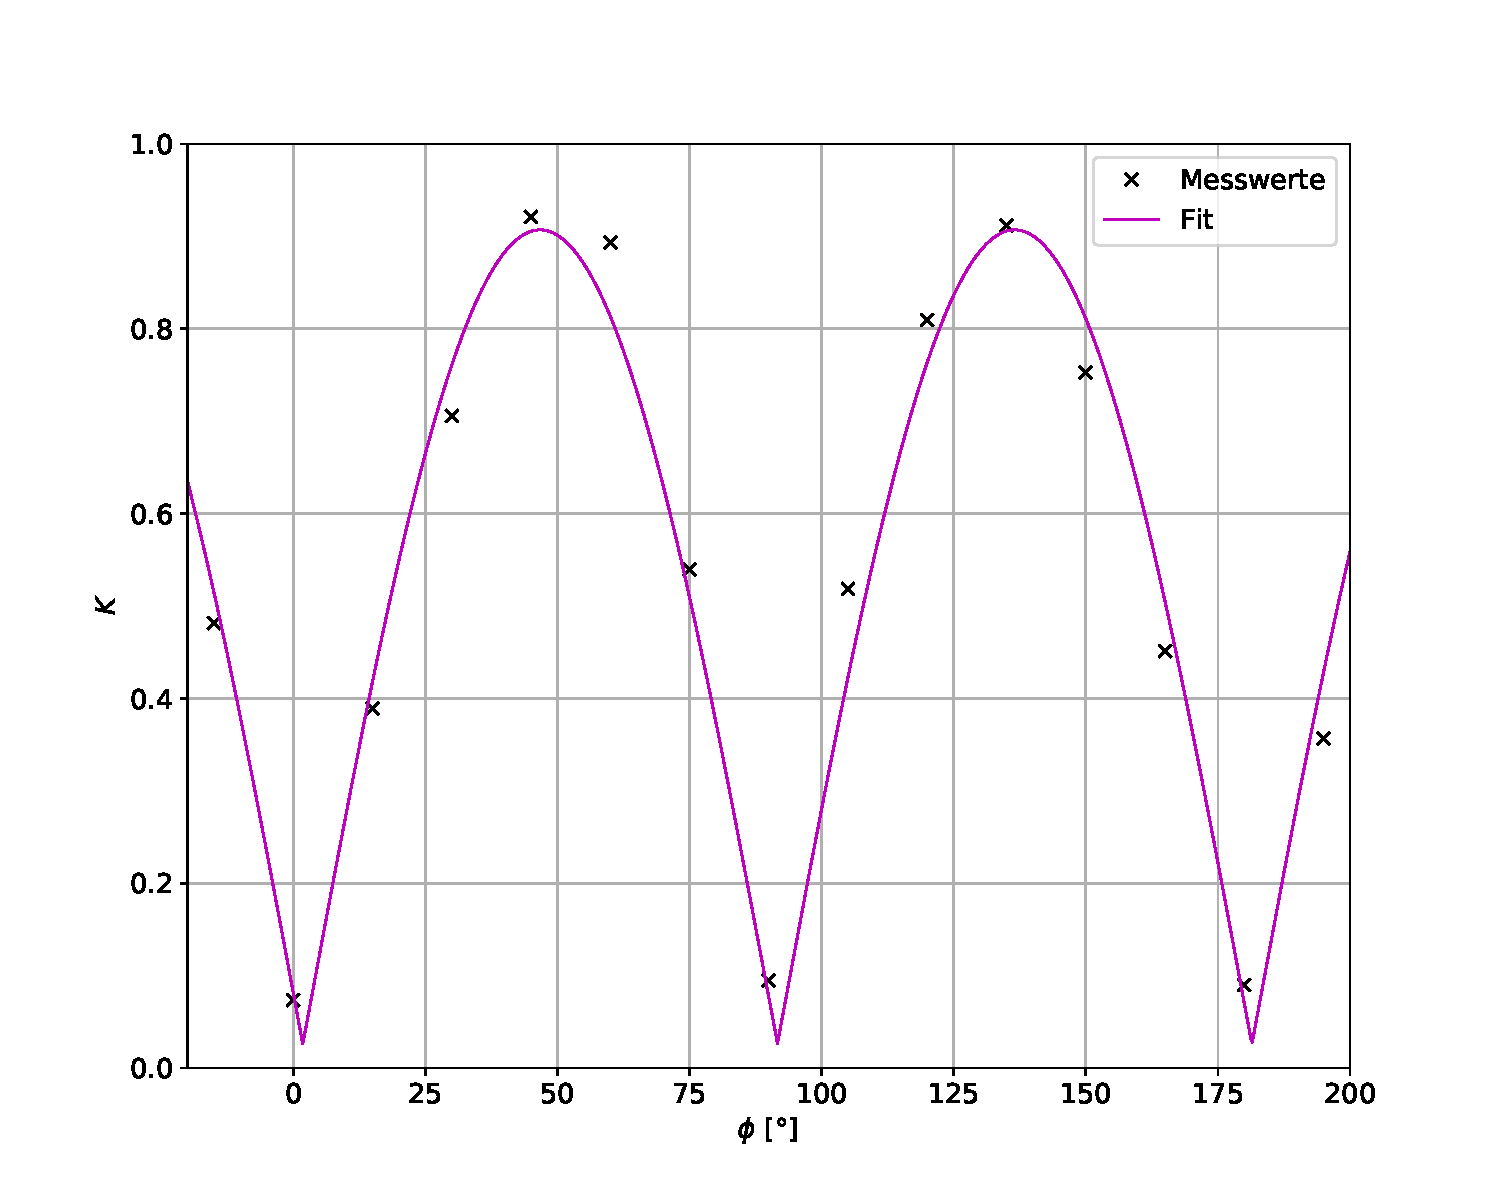
\includegraphics[width=\textwidth]{kontrast.pdf}
  \caption{Kontrast in Abhängigkeit der Polarisationsrichtung mit
  Ausgleichsrechnung}
  \label{fig:kontrast}
\end{figure}
\subsection{Berechnung des Brechungsindex von Glas}
\begin{table}

  \centering
\begin{tabular}{SSSSSS}

  \toprule
  \multicolumn{2}{c}{Messung 1} &\multicolumn{2}{c}{Messung 2}
  & \multicolumn{2}{c}{Messung3} \\
$\phi \, [\si{\radian}]$ & $M$ & $\phi \, [\si{\radian}]$ & $M$ &
 $\phi \, [\si{\radian}]$ & $M$ \\

 \midrule
2 & 6 & 2 & 6 & 2 & 5 \\

2 & 7 & 2 & 7 & 2 & 6 \\

2 & 8 & 2 & 7 & 2 & 8 \\

2 & 7 & 2 & 6 & 2 & 7 \\

2 & 6 & 2 & 7 & 2 & 6 \\

\bottomrule
\end{tabular}
\caption{Gemessene Anzahl der Maxima pro Winkeländerung}

\label{tab:glas}
\end{table}


\subsection{Berechnung des Brechungsindex von Luft}

Für die Messungen des Brechungsindex von Luft ergeben sich folgende Werte
\begin{align*}
  \text{Messung 1} &= 42 \text{Counts} \\
  \text{Messung 2} &= 42 \text{Counts} \\
  \text{Messung 3} &= 42 \text{Counts} \, . \\
\end{align*}
Es muss beachtet werden, dass kein vollständiges Vakuum erreicht werden konnte
und das der Wert des erreichten Normaldrucks nicht dem üblichen Wert von
$p_a= \SI{1013}{\milli\bar}$ entspricht. Die erreichten Druckwerte sind in
diesem Versuch die Folgenden.
\begin{align*}
  p_{\text{min}} &= \SI{1002}{\milli\bar} \\
  p_0            &= \SI{5}{\milli\bar} \\
\end{align*}

Zur Berechnung des Brechungsindes von Luft wird Formel \ref{eqn:brechluft}
verwendet. Die Länge der Messzelle $L$ und die Wellenlänge des Lasers
haben dabei die folgenden Werte.

\begin{align*}
  L &= \SI{100 \pm 0.1}{\milli\meter} \\
  \lambda &= \SI{632.990}{\nano\meter} \\
\end{align*}

Dadurch ergeben sich für die einzelnen Messung die folgenden Brechunsindizes.
\begin{align*}
  n_1 &= 1.0001 \\
  n_2 &= 1.0001 \\
  n_3 &= 1.0001 \\
\end{align*}
Wird lediglich der Fehler der Messzelle berücksichtig, so ergibt sich mittels
Gaußscher Fehlerfortpflanzung ein Wert von
\begin{align*}
  n = 1.0001 \pm (1.3 \cdot 10^{-7}) \\
\end{align*}
